\chapter{Modelos} \label{chp:models}

%%%%%%%%%%%%%%%%%%%%%%%%%%%%%%%%%%%%%%%%%%%%%%%%%%%%%%%%%%%%%%%%%%%%%%%%%%%%%%%%
%%%%%%%%%%%%%%%%%%%%%%%%%%%%%%%%%%%%%%%%%%%%%%%%%%%%%%%%%%%%%%%%%%%%%%%%%%%%%%%%

\begin{figure}[htbp]
\centering
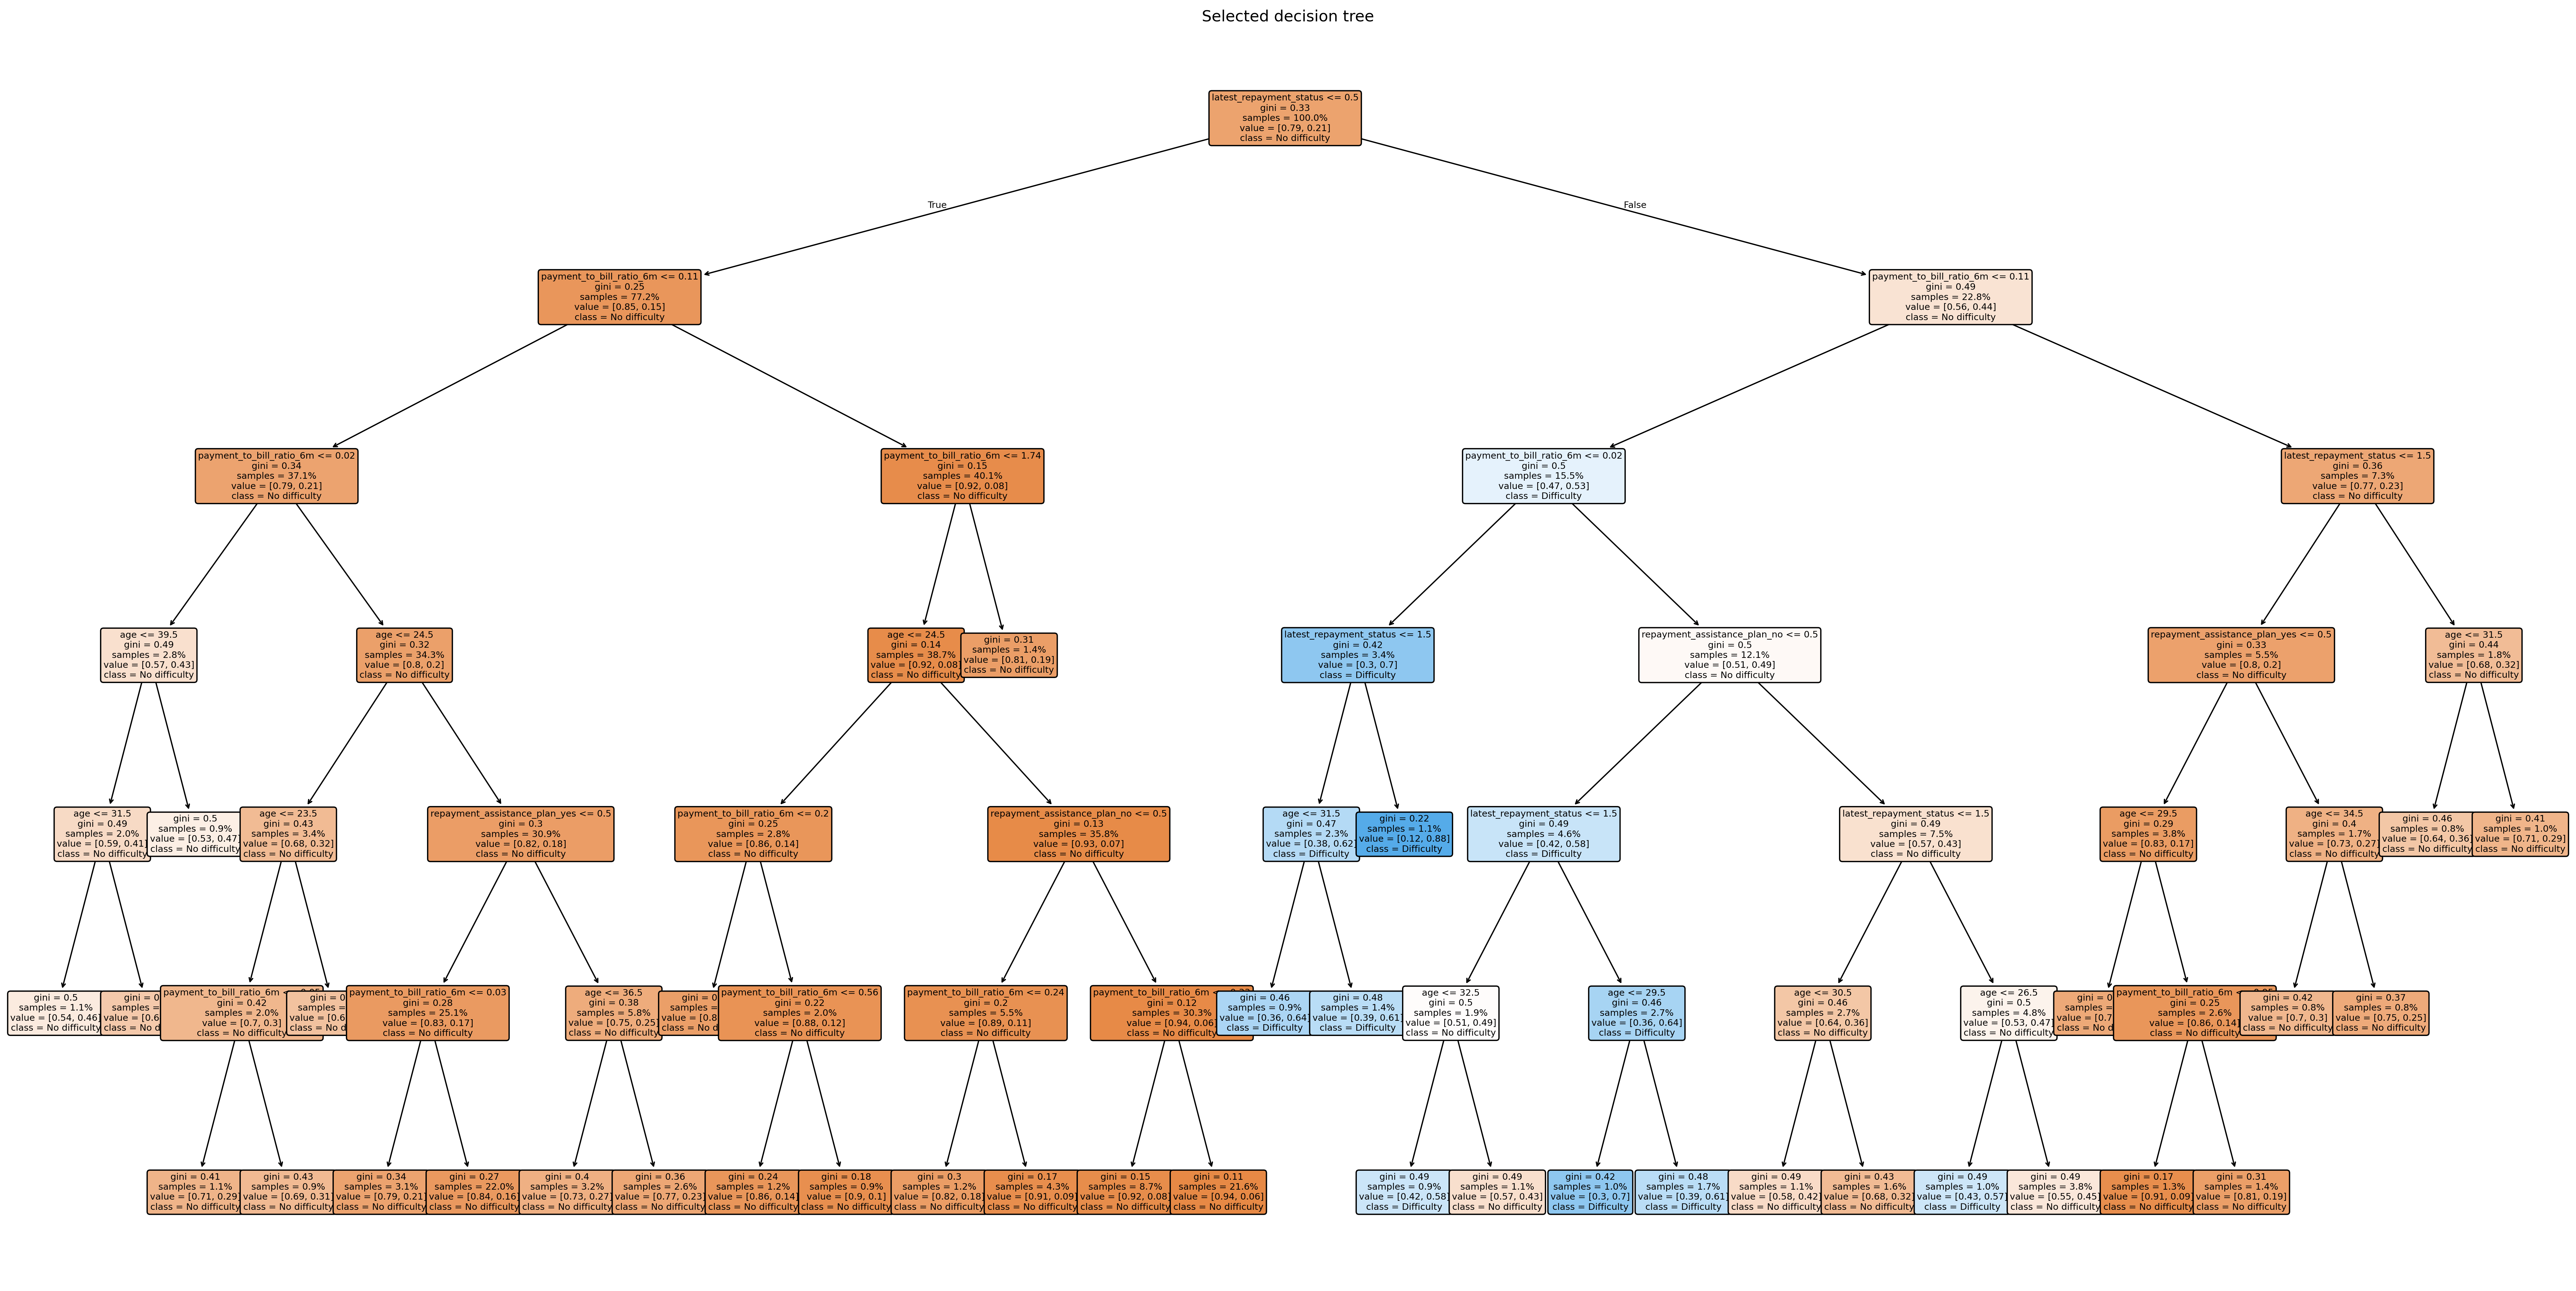
\includegraphics[width=0.9\textwidth]{images/figure_09.png}
\caption{Árbol de decisión final. Cada nodo muestra la condición de división,
la impureza de Gini, el porcentaje de muestras y la distribución de clases;
cada hoja indica la clase predicha.}
\label{fig:final-tree}
\end{figure}

\section{Interpretación global del árbol}

La figura \ref{fig:final-tree} muestra el árbol final, cuya estructura se
interpreta a continuación.

El árbol tiene profundidad dos y exige al menos 200 observaciones por hoja. Su
comportamiento se apoya únicamente en dos variables de comportamiento de pago:
\texttt{latest_repayment_status}, con una importancia basada en impureza de
0.655, y \texttt{payment_to_bill_ratio_6m}, con 0.345 (figura
\ref{fig:feature-importance}). Esta ordenación describe el uso que el modelo
hace de las variables, no una relación causal.

\begin{figure}[htbp]
\centering
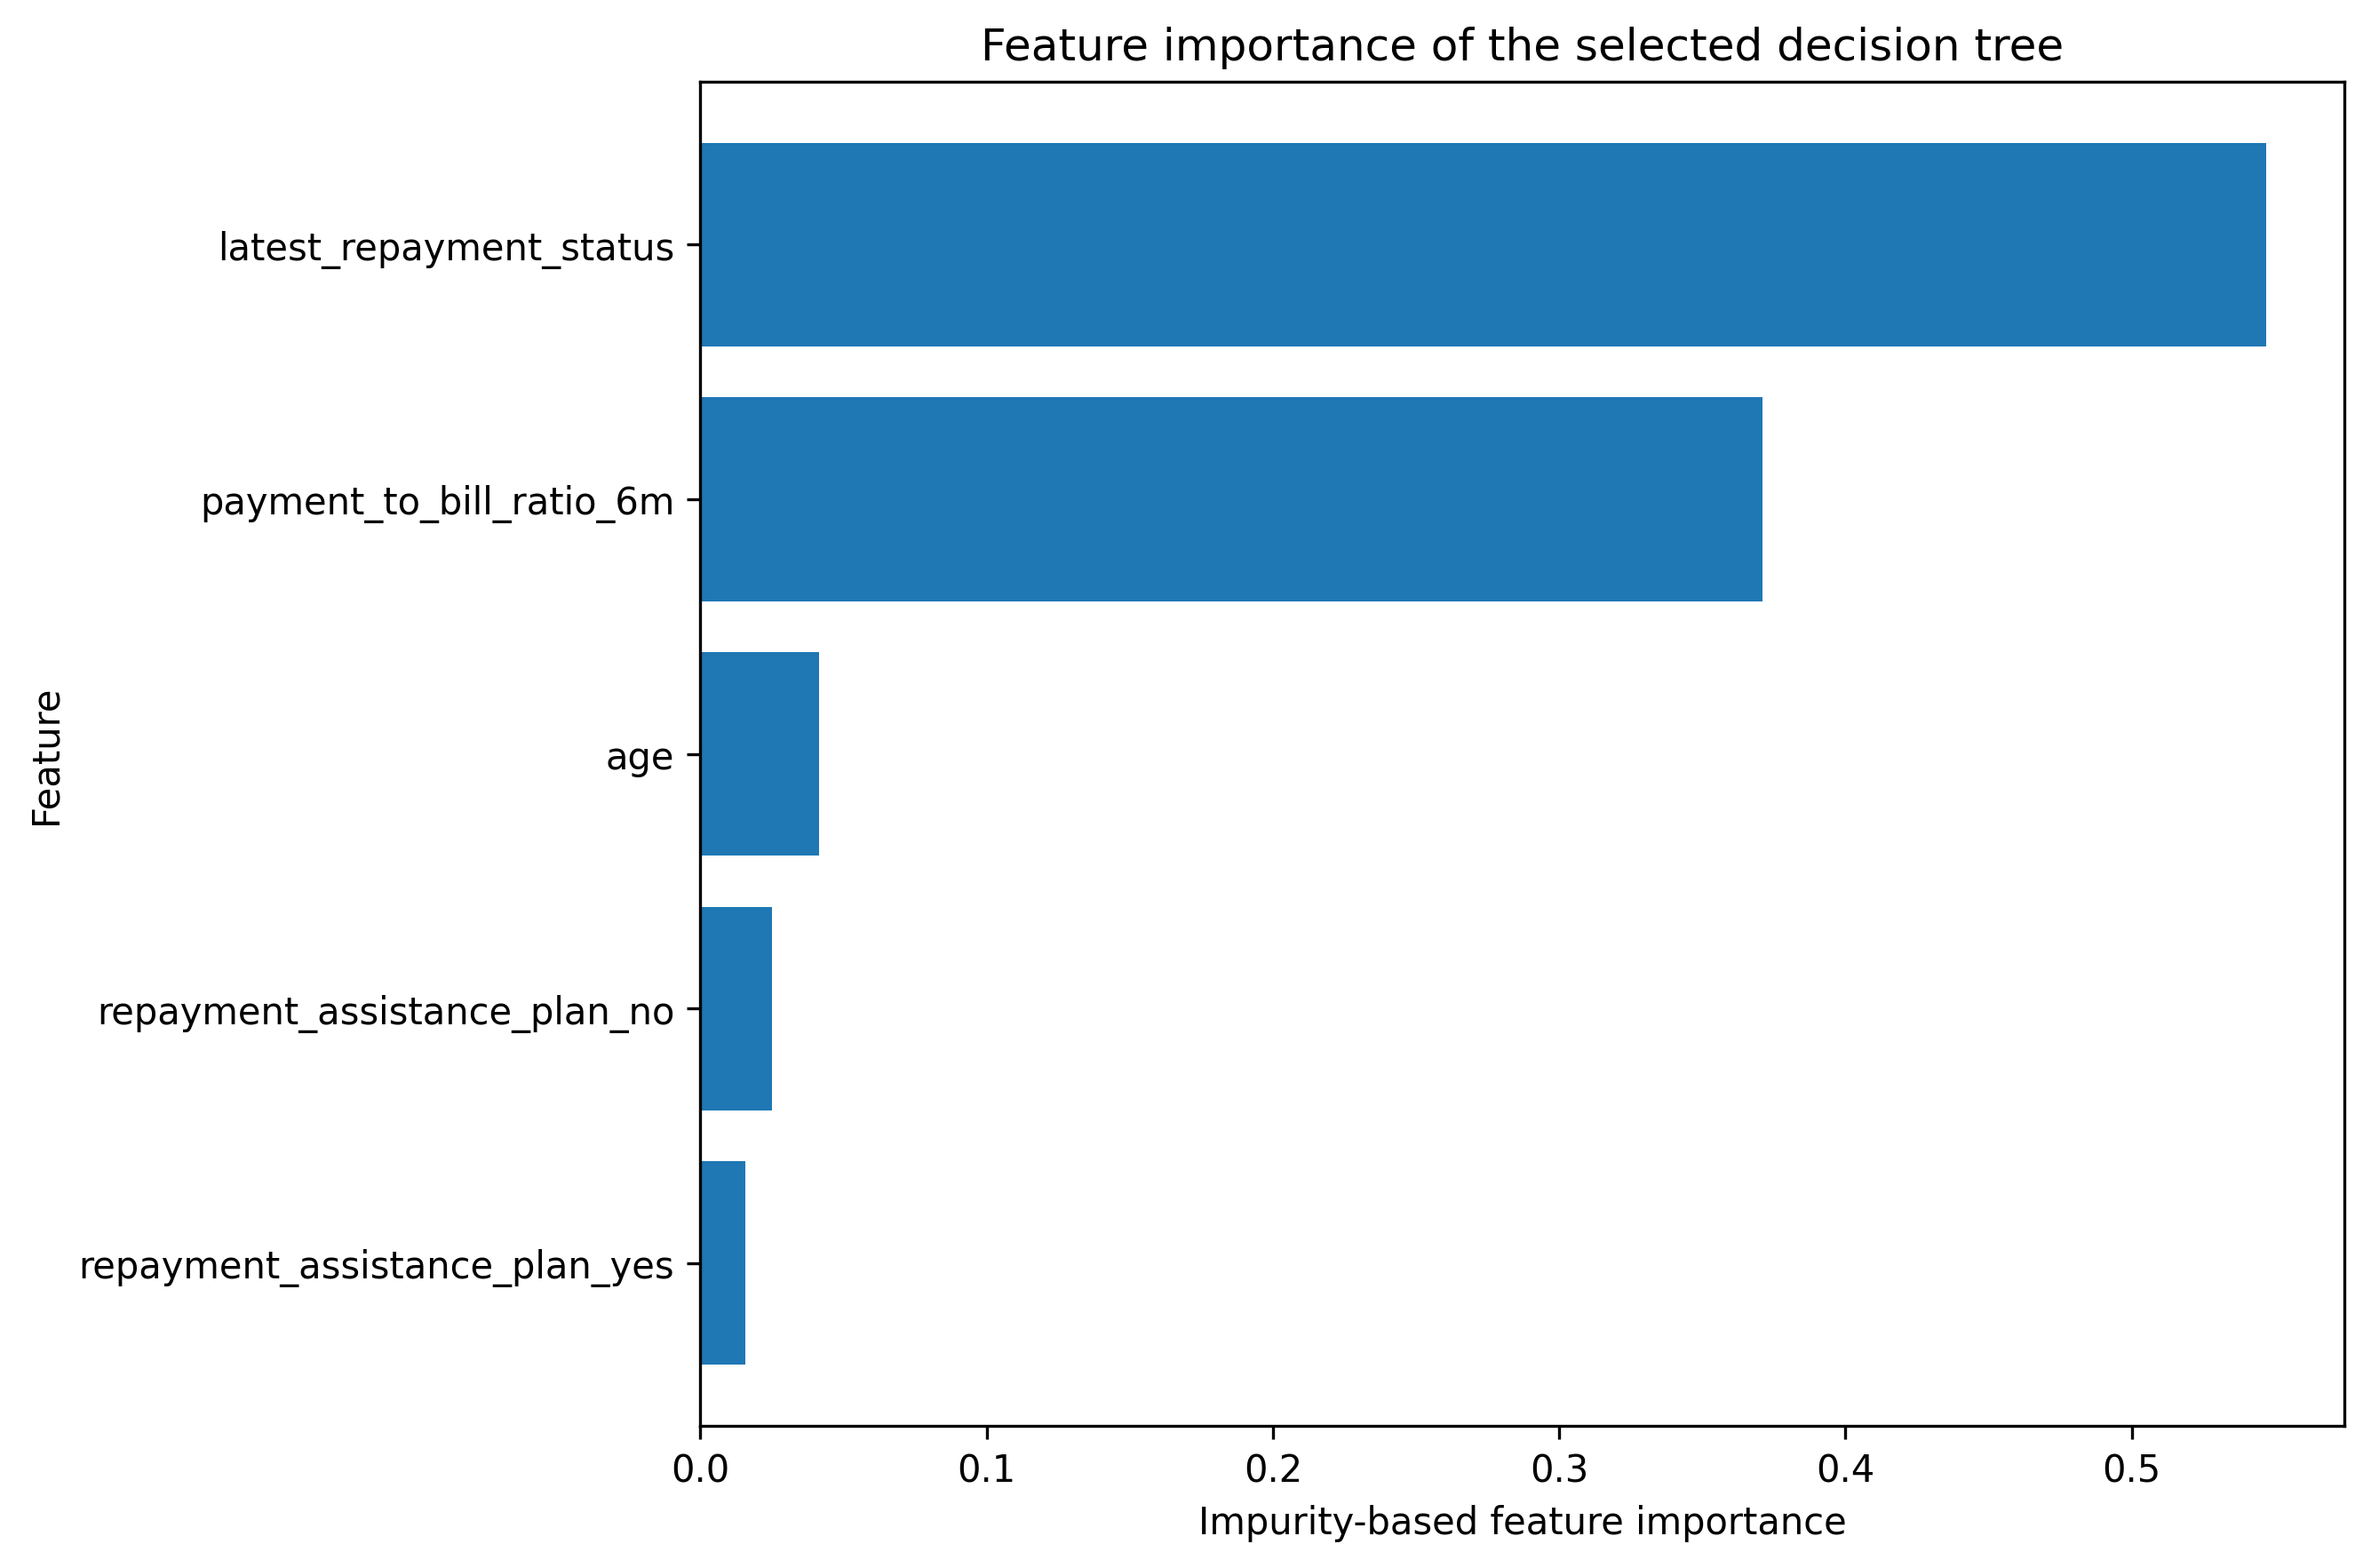
\includegraphics[width=0.75\textwidth]{images/figure_08.png}
\caption{Importancia basada en impureza de las variables usadas por el árbol
final.}
\label{fig:feature-importance}
\end{figure}

La raíz divide según \texttt{latest_repayment_status} en 0.5. Si el estado de
devolución es bajo (0.5 o menos), ambas hojas predicen ausencia de dificultad,
con probabilidades estimadas de 0.215 o 0.081 según el ratio de pago. Si el
estado es alto (más de 0.5), el modelo distingue después según
\texttt{payment_to_bill_ratio_6m} en 0.105: la hoja con ratio bajo concentra
la mayor probabilidad de dificultad (0.535), mientras que la hoja con ratio alto
baja a 0.233. Las hojas terminales asignan la clase mayoritaria de las
observaciones que alcanzan cada región y usan su frecuencia de clase 1 como
probabilidad estimada. Así, el modelo puede leerse como una colección de reglas, ya que
una observación sigue una secuencia de condiciones hasta una hoja y recibe la
probabilidad de dificultad observada en esa hoja.

Las hojas extremas resumen el comportamiento del modelo. La hoja de mayor riesgo
(nodo 5) corresponde a \texttt{latest_repayment_status} $>$ 0.5 y
\texttt{payment_to_bill_ratio_6m} $\leq$ 0.105, con una probabilidad estimada de
clase 1 de 0.535 y 3\,875 observaciones. La de menor riesgo (nodo 3) corresponde
a \texttt{latest_repayment_status} $\leq$ 0.5 y
\texttt{payment_to_bill_ratio_6m} $>$ 0.105, con 0.081 y 10\,027 observaciones
(figura \ref{fig:leaf-probabilities}).

\begin{figure}[htbp]
\centering
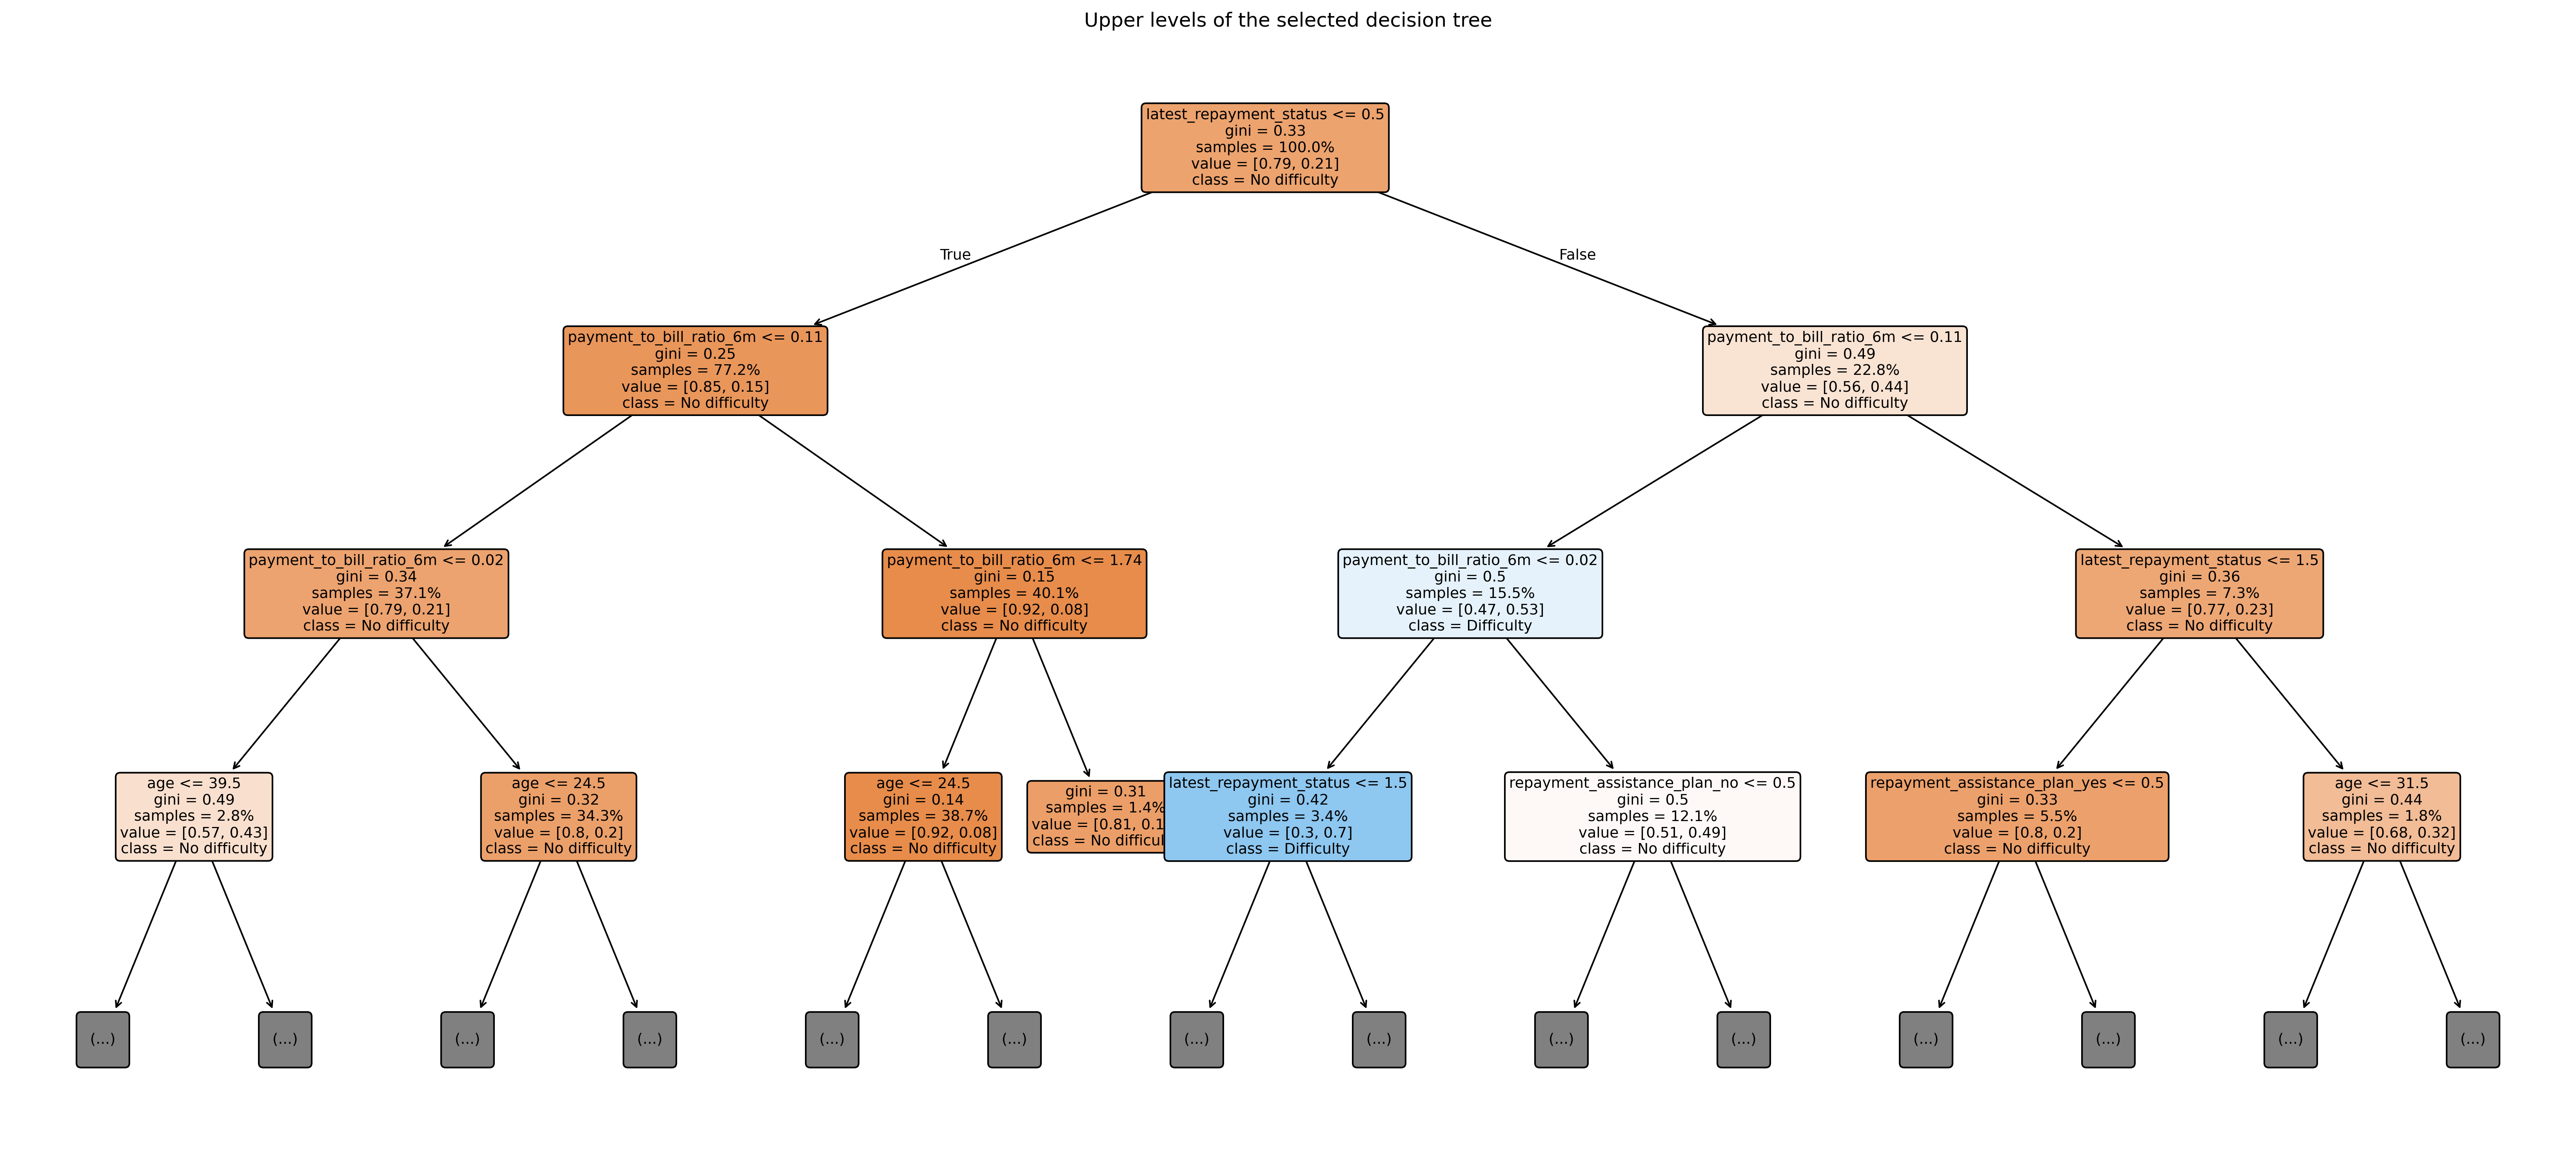
\includegraphics[width=0.75\textwidth]{images/figure_10.png}
\caption{Probabilidad estimada de dificultad en cada hoja terminal, ordenadas
por riesgo, junto con la tasa positiva global.}
\label{fig:leaf-probabilities}
\end{figure}

Estas reglas describen asociaciones del predictor, no causas del impago. Por
ello, que el árbol asocie determinados perfiles de pago con mayor riesgo no
permite concluir que las variables provoquen la dificultad posterior.

\section{Explicaciones locales}

Se conservaron dos observaciones correctamente clasificadas mediante
predicciones out-of-fold, una de cada clase. Para \texttt{CR26-125466}, cuya
clase real es 1, el árbol estima una probabilidad de aproximadamente 0.233 y,
con el umbral seleccionado de 0.09, la clasifica como dificultad (con el umbral
por defecto de 0.5 se clasificaría como ausencia). Su camino es
\texttt{latest_repayment_status} $>$ 0.5 y
\texttt{payment_to_bill_ratio_6m} $>$ 0.105. Para \texttt{CR26-103063}, cuya
clase real es 0, estima una probabilidad de clase 1 de aproximadamente 0.081 y
la clasifica como ausencia de dificultad tanto con 0.5 como con 0.09; su camino
es \texttt{latest_repayment_status} $\leq$ 0.5 y
\texttt{payment_to_bill_ratio_6m} $>$ 0.105.

La explicación de cada caso es su camino desde la raíz hasta la hoja terminal:
las condiciones sobre las dos variables seleccionadas se combinan, y la
probabilidad de la hoja resume la proporción de casos positivos en esa región.
Las figuras \ref{fig:path-positive} y \ref{fig:path-negative} muestran el árbol
con el camino recorrido por cada observación resaltado.

\begin{figure}[htbp]
\centering
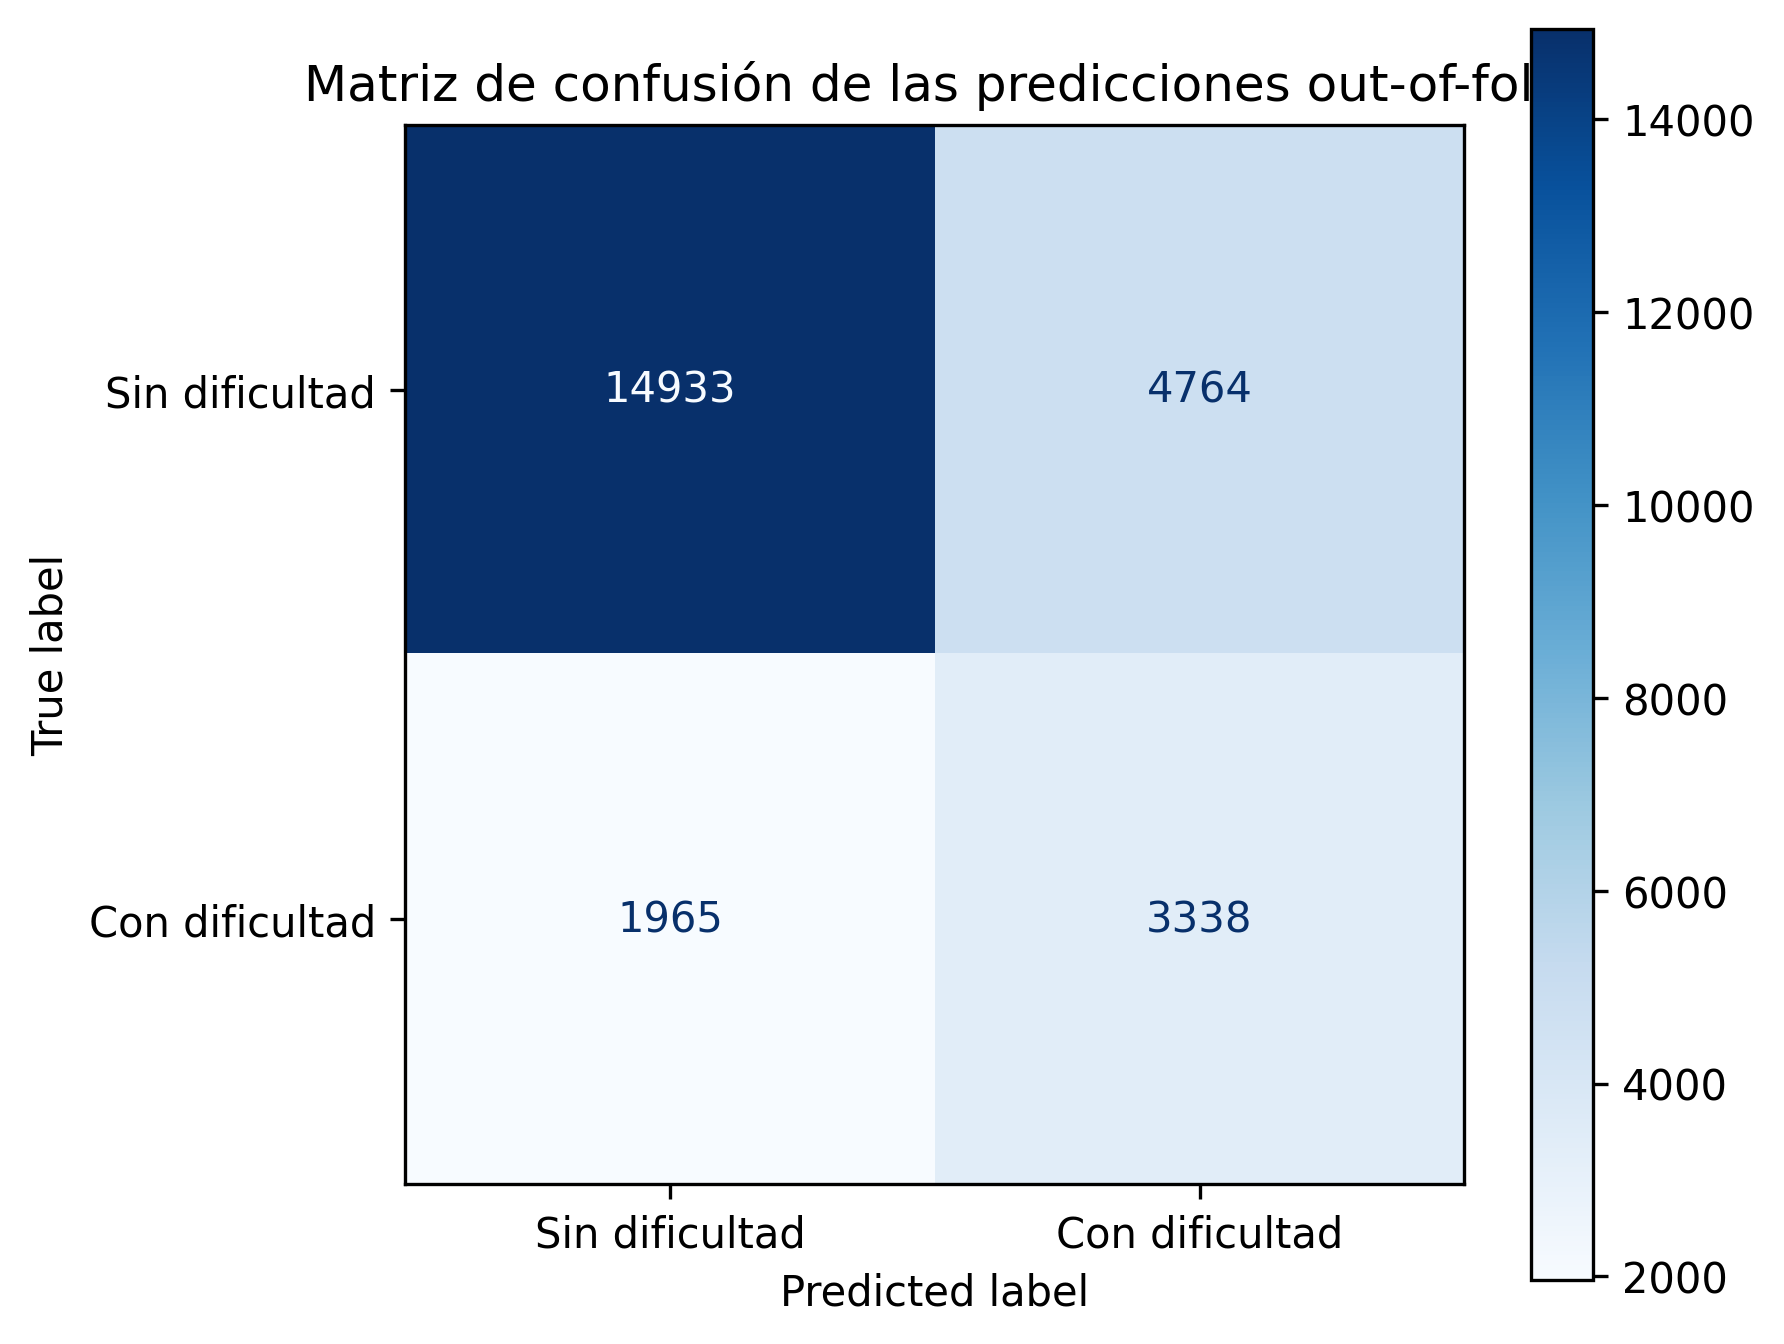
\includegraphics[width=0.95\textwidth]{images/figure_14.png}
\caption{Camino de decisión de CR26-125466 (clase real 1) resaltado
sobre el árbol final.}
\label{fig:path-positive}
\end{figure}

\begin{figure}[htbp]
\centering
\includegraphics[width=0.95\textwidth]{images/figure_15.png}
\caption{Camino de decisión de CR26-103063 (clase real 0) resaltado
sobre el árbol final.}
\label{fig:path-negative}
\end{figure}

Los caminos de decisión no cambian al modificar el umbral, ya que este solo
convierte la probabilidad estimada de la hoja en una clase. Esta forma de
explicación es directamente verificable y adecuada para un modelo lógico, aunque
no implica que cada condición aislada sea suficiente ni causal. Los mismos casos
se utilizarán con logística y EBM en la entrega final para comparar
explicaciones.
